\documentclass{standalone}
\usepackage{graphicx}	
\usepackage{amssymb, amsmath, amsthm}
\usepackage{color}

\usepackage{tikz}
\usetikzlibrary{intersections, backgrounds, math}

\definecolor{light}{RGB}{220, 188, 188}
\definecolor{mid}{RGB}{185, 124, 124}
\definecolor{dark}{RGB}{143, 39, 39}
\definecolor{highlight}{RGB}{180, 31, 180}
\definecolor{lightteal}{RGB}{107, 142, 142}
\definecolor{midteal}{RGB}{72, 117, 117}
\definecolor{darkteal}{RGB}{29, 79, 79}
\definecolor{darkolive}{RGB}{97, 123, 45}
\definecolor{gray10}{gray}{0.1}
\definecolor{gray20}{gray}{0.2}
\definecolor{gray30}{gray}{0.3}
\definecolor{gray40}{gray}{0.4}
\definecolor{gray60}{gray}{0.6}
\definecolor{gray70}{gray}{0.7}
\definecolor{gray80}{gray}{0.8}
\definecolor{gray90}{gray}{0.9}
\definecolor{gray95}{gray}{0.95}

\begin{document}

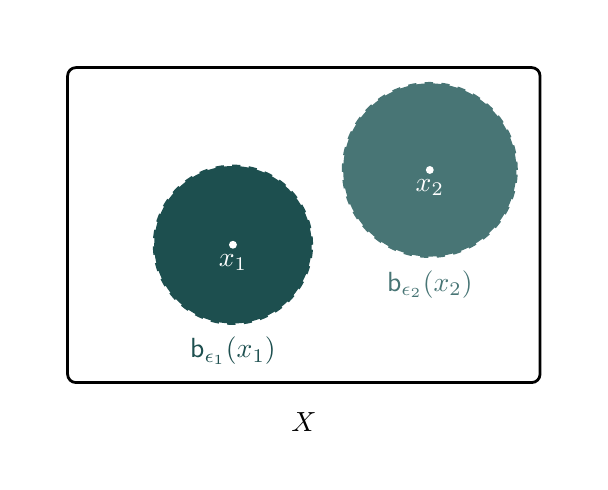
\begin{tikzpicture}[scale=1.0]
  
  \draw[white] (-3.5, -3) rectangle (3.5, 2.5);

  \draw[rounded corners=3, color=black, line width=1] (-3, -2) rectangle (3, 2);
  \node at (0, -2.5) { $X$ };

  \filldraw[darkteal, dashed, line width=1] (-0.9, -0.25) circle (1); 
  \node[darkteal] at (-0.9, -1.6) {$\mathsf{b}_{\epsilon_{1}}(x_{1})$};
  \fill[white] (-0.9, -0.25) circle (0.05) node[below] { $x_{1}$ };
  
  \filldraw[midteal, dashed, line width=1] (1.6, 0.7) circle (1.1); 
  \node[midteal] at (1.6, -0.75) {$\mathsf{b}_{\epsilon_{2}}(x_{2})$};
  \fill[white] (1.6, 0.7) circle (0.05) node[below] { $x_{2}$ };
    
\end{tikzpicture}

\end{document}  